\documentclass[10pt]{report}

\usepackage{pgfplots}
\pgfplotsset{compat=1.18}
\usepackage{amsmath}
\usepackage{dirtytalk}
\usepackage{graphicx}
\graphicspath{ {./Images/} }
\usepackage{tikz}
\usepackage[T1]{fontenc}
\usepackage{lmodern}
\usepackage{fancyhdr}
\pagestyle{fancy}
\usepackage{caption}
\usepackage{multicol}
\fancyhf{}
\fancypagestyle{plain}{
    \fancyhf{}
    \fancyfoot[C]{\thepage}
    \renewcommand{\headrulewidth}{0pt}
    \renewcommand{\footrulewidth}{0pt}
}
\renewcommand{\headrulewidth}{0pt}
\pagestyle{fancy}
\usepackage[a4paper, top=0in, margin=1in]{geometry}
\fancyfoot[C]{\thepage}
\usepackage{parskip}
\usepackage{hyperref}
\hypersetup{
    colorlinks=true,
    linkcolor=black,
    filecolor=magenta,
    urlcolor=cyan
    }
\usepackage{titlesec}
\usepackage{float}
\usepackage{subfig}

\usepackage[style=ieee]{biblatex}
\addbibresource{references.bib}

\titleformat{\chapter}[display]
  {\normalfont\huge\bfseries}{\chaptertitlename\ \thechapter}{0pt}{\Huge}
\titlespacing*{\chapter}{0pt}{0pt}{10pt}

\newcommand{\includegraphicsrounded}[3]{
    \begin{tikzpicture}
        \clip[rounded corners=1em] (0,0) rectangle node {\includegraphics[width=#2,height=#3]{#1}} (#2,#3);
    \end{tikzpicture}
}

\title{
    \bfseries
    \includegraphicsrounded{figures/title.png}{12cm}{10cm} \\
    \vspace{1cm}
    \large{Deep Learning on Images and Signals} \\
    \LARGE{U-Nets in a Self-Driving Segmentation Task} \\
}

\author{
    Nils Fahrni \\
    \small{BSc Data Science Student}
    }
\date{\today}

\begin{document}

\maketitle

\tableofcontents

\chapter{Task}

\section{Research Question}

The research question which I aim to answer with this mini-challenge is: 

\say{How does the performance of a U-Net semantic segmentation model differ between scenes of city streets and non-city streets in the BDD100K dataset?}

This research question is interesting because it addresses the practical challenges of deploying semantic segmentation models in real-world applications, such as autonomous driving, where environmental variability is a key concern. City and non-city environments differ significantly in terms of visual characteristics, object density, and lighting conditions, which can impact the performance of computer vision models.

\section{Dataset}

I decided for the BDD100K dataset. The BDD100K dataset is the largest driving video dataset, featuring 100,000 videos and supporting 10 tasks for evaluating and advancing multitask learning in autonomous driving. It offers diverse geographic, environmental, and weather conditions, making it a benchmark for studying heterogeneous multitask learning and training robust computer vision models \cite{yuBDD100KDiverseDriving2020}. 

For this Mini Challenge I use the "10k" subset, which is made up of 10,000 RGB images and are sampled from the 100,000 videos' frames. This subset is intended for semantic segmentation tasks. These 10,000 images have already been pre-partitioned into a train, validation and test partition. The train partition consists of 8000 images, the validation 1000 and the test 1000.

This smaller subset does unfortunately not have scene attributes but the larger video dataset does. Since the semantic segmenatiton subset is derived from the video dataset, I retrieve the scene attributes through the larger datasets metadata JSON. The issue here is that not all images in the semantic segmentation subset seem to be in the video dataset. I will therefore only use the small overlap of images that has scene attributes and exists both in the video and semantic segmentation dataset. This overlap consists of 3426 images.

\section{Methodology and Procedure}
To answer the research question, I will train a \textbf{U-Net} model on the BDD100K dataset. The U-Net architecture is a common choice for segmentation tasks as it contains an Encoder-Decoder structure:
\begin{enumerate}
    \item \textbf{Encoder}: Extracts features from the input image using a series of convolutional and downsampling operations, capturing contextual information. The downsampling path in the encoder captures features at multiple scales, enabling the model to understand both local and global context. This is essential in self-driving tasks to distinguish between small objects (like traffic cones) and large areas (like the road).
    \item \textbf{Decoder}: Gradually upsamples the feature maps and uses convolutions to predict dense segmentation maps. This structure is ideal for segmenting objects in self-driving scenarios, such as lanes, vehicles, pedestrians, and road signs.
\end{enumerate}

As a second model I will modify the U-Net model to include an attention mechanism, which I will implement myself according to \cite{oktayAttentionUNetLearning2018}. I expect the addition of attention to be another improving factor because:
\begin{enumerate}
    \item \textbf{Driving Reality}: Different objects and their spatial relationships often define the context. For instance:
    \begin{enumerate}
        \item  A cyclist is more likely to be found near a bike lane or the edge of a road.
        \item A pedestrian might be near a crosswalk but not in the middle of a highway.
        Cars and trucks are expected on roads but not sidewalks.
    \end{enumerate} 
    \item \textbf{Attention Benefit}: The attention mechanism allows the model to focus not just on isolated objects but also on the relationships between them. It helps the network infer that the presence of a bike lane increases the likelihood of a cyclist or that highway lanes imply the absence of pedestrians and cyclists.
\end{enumerate}

I will then evaluate the models on the test set and compare the performance between city street and non-city street scenes. To measure and evaluate the performance between different model complexities numerically, I will use the mean Intersection over Union (mIoU) as the evaluation metric.

Both models will be explored within the schema of "A Recipe for Training Neural Networks" according to Andrej Karpathy \cite{karpathyRecipeTrainingNeural2019}.
\chapter{Discussion}

\section{Answering The Research Question}
To answer if the models answer the research question in a satisfactory manner I have calculated the Intersection over Union (IoU) metric for both city scene images and non-city scene images from the held out test datset. This allows me to compare the main metric between all explored models. Here I show the winner models from all explorations in the training process:

\begin{figure}[h] 
    \centering 
    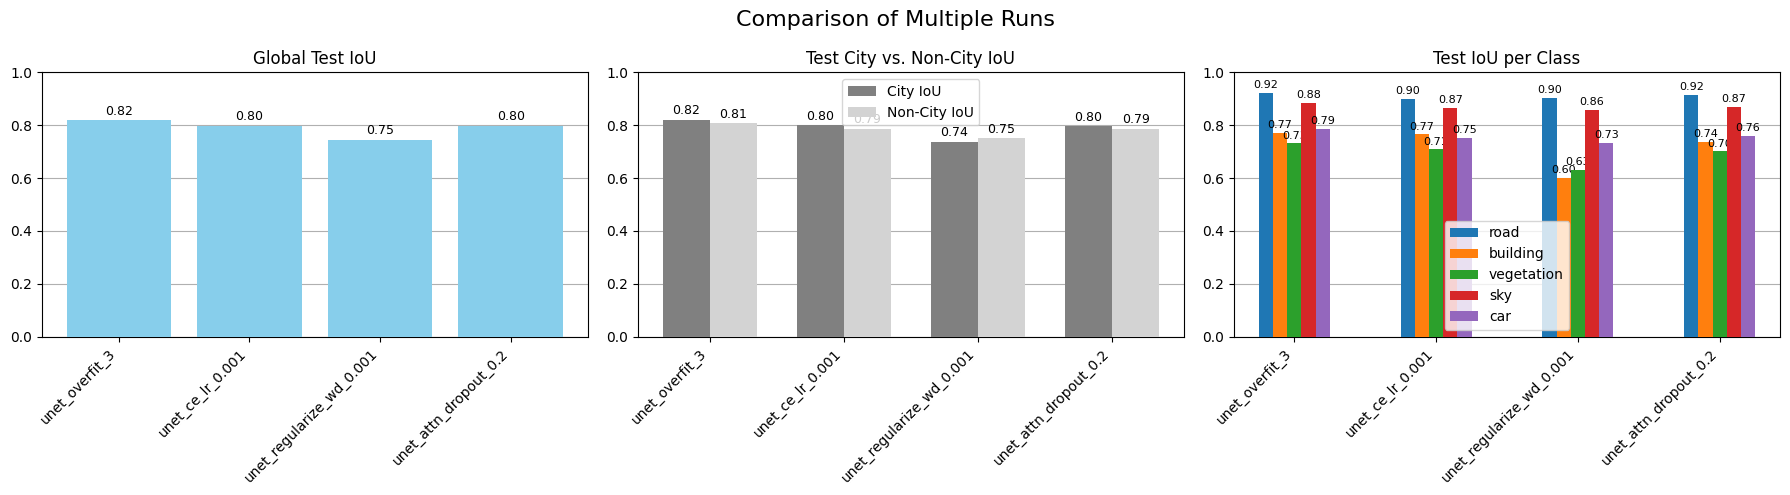
\includegraphics[width=0.8\textwidth]{figures/winners_comparison.png} 
    \caption{Comparison of the winner models.} 
    \label{fig:winners_comparison} 
\end{figure}

The center subplot shows the mentioned comparison of non-city scene and city scene IoUs. When it comes to numerical analysis exclusively, the Vanilla U-Net (here, named \texttt{unet\_overfit\_3}) performed the best. This model is expected to overfit, however only the lowest validation loss weights get saved, thus, we do not necessarily see "bad" results as the model was saved at a state where it generalizes well. 

Upon further visual inspection, the Attention U-Net with Dropout regularization also performed quite well. It has has slightly lower IoU metrics than the Vanilla U-Net with \texttt{128} base filters (\texttt{unet\_overfit\_3}) but seems to visually get more details correct in more difficult environments.

To answer the research question, the models are undoubtedly capable of performing well in both types of scenes. There is no significant difference between both recorded metrics. Thus, the models are not clearly biased towards one scene or have a clear deficit towards one direction.

\section{Chances and Risks}
Here I will discuss the challenges and risks of the proposed models and the approach behind them:

\noindent
\begin{minipage}{0.44\textwidth}
    \subsubsection*{Chances} 
    \begin{itemize} 
        \item[+] With this mini challenge I present a clear framework of components that would allow for a streamlined exploration of further models and hyperparameters.
        \item[+] Looking at the results, the models did succeed in the most critical classes like \texttt{road} and \texttt{car} which are essential for systems that require lane holding and collision avoidance.
        \item[+] The models at hand are derived from a well-known architecture, the U-Net which is simple but yet reached quite good results.
    \end{itemize} 
\end{minipage}
\hspace{0.05\textwidth}
\begin{minipage}{0.44\textwidth}
    \subsubsection*{Risks} 
    \begin{itemize} 
        \item[-] The models were trained on a limited dataset, with less than 3500 images and only the 5 largest classes.
        \item[-] Sampling from the models can take a long time with the larger models proposed which is not ideal for real-time applications like self-driving.
        \item[-] The handling of classes in the images that were removed for training were not labeled into a clear "background class" so the model learned to assign one of the 5 most common classes to those objects. 
    \end{itemize} 
\end{minipage}

\section{Comparing The Models}
To conclude the steps that included training of the Machine Learning Recipe proposed by \textcite{karpathyRecipeTrainingNeural2019}, I compared all models of their corresponding step. Here are these interim results:

\subsection{Overfitting Experiments}

\begin{figure}[h] 
    \centering 
    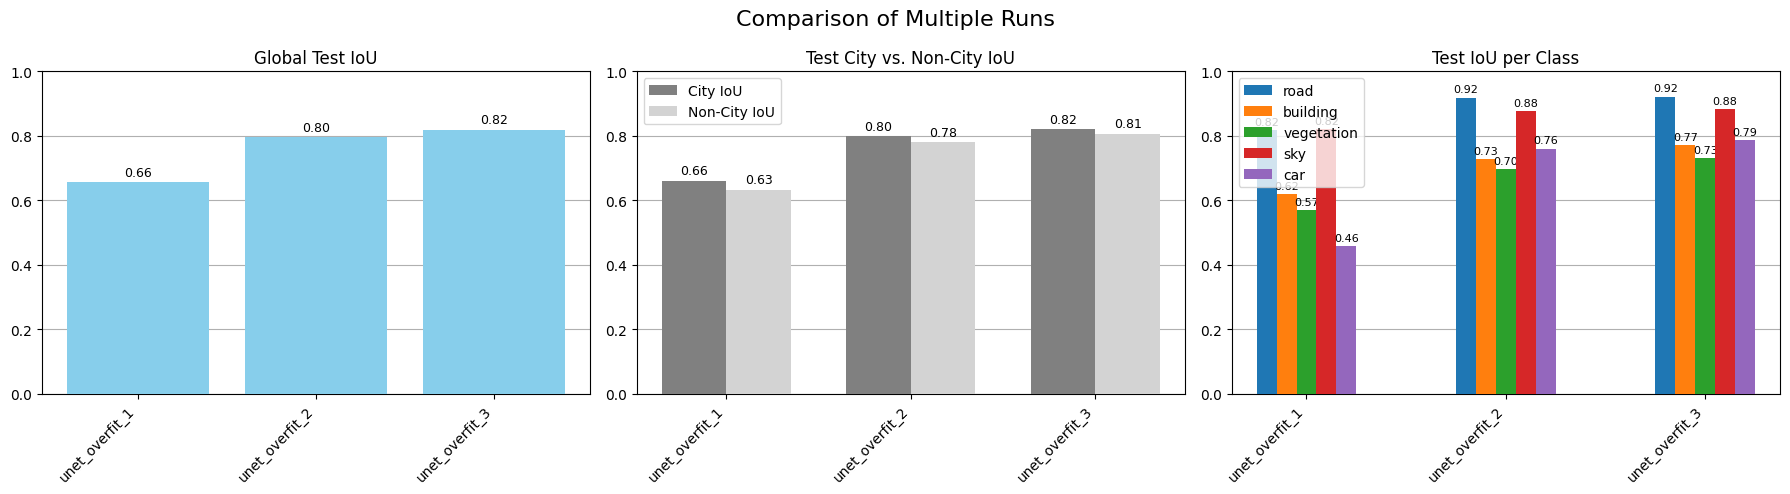
\includegraphics[width=0.8\textwidth]{figures/overfit_comparison.png} 
    \caption{Comparison of the models explored in the Overfitting Phase.}
    \label{fig:overfit_comparison} 
\end{figure}

In the overfit experiments I have gradually increased complexity by adding more base filters to the Vanilla U-Net. The results showed that the model benefits from a higher complexity - The highest increase happened between \texttt{32} and \texttt{64} base filters. The model with \texttt{128} base filters performed the best in the overfitting experiments.

\subsection{Regularization Experiments}

\begin{figure}[h] 
    \centering 
    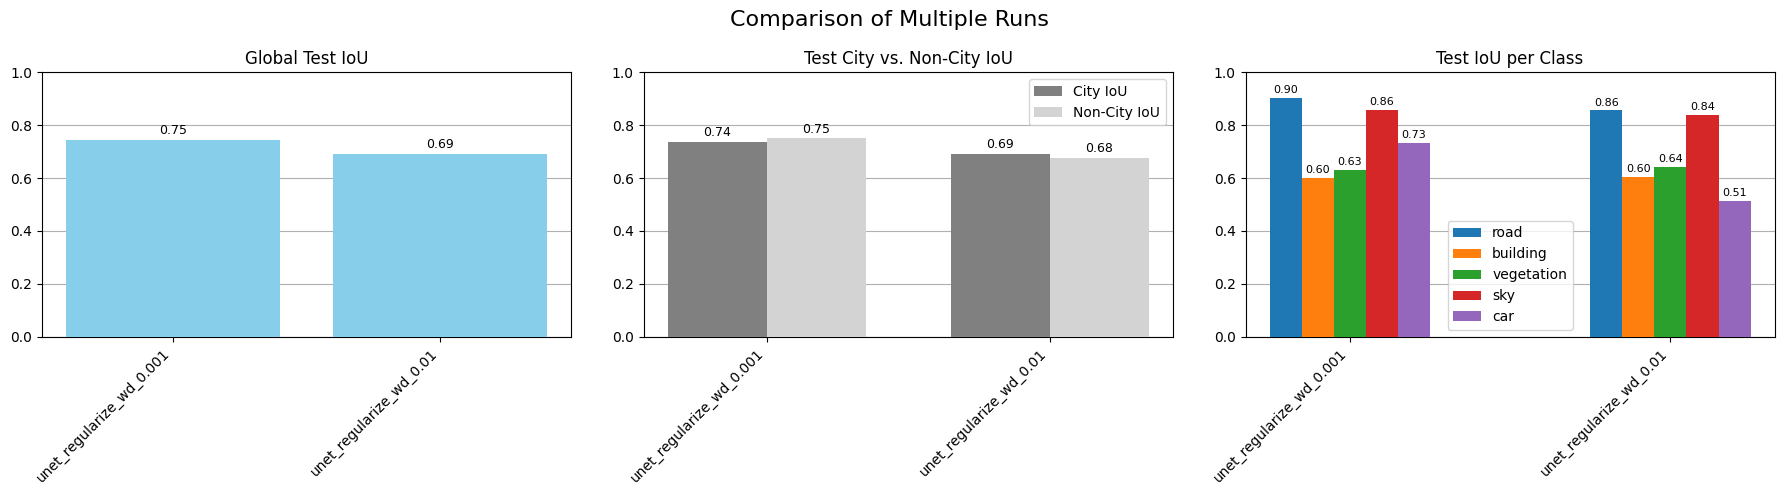
\includegraphics[width=0.8\textwidth]{figures/regularization_comparison.png} 
    \caption{Comparison of the models explored in the Regularization Phase.} 
    \label{fig:regularization_comparison} 
\end{figure}

During regularization I only explored different \texttt{weight\_decay} parameters. I believe there is still some potential to explore other regularization techniques with the Vanilla U-Net. I have later on explored Dropout regularization with the Attention U-Net which looked more promising in regards to the loss curves.

\subsection{Hyperparameter Tuning}

\begin{figure}[h] 
    \centering 
    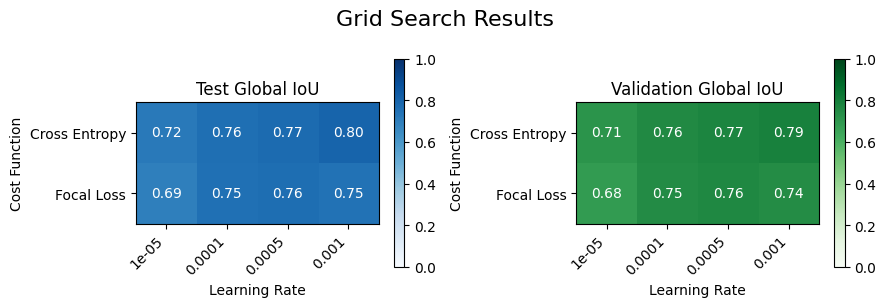
\includegraphics[width=0.8\textwidth]{figures/grid_search.png} 
    \caption{Comparison of the models that went through Grid Search.} 
    \label{fig:grid_search} 
\end{figure}

I also wanted to implement the Focal Loss error function so that presented itself as a good hyperparameter to explore. Ultimately, what resulted was that the Focal Loss may be too nuanced for this dataset as there is no acute imbalance between the classes so a more classical loss function like the Weighted Cross Entropy turned out to work better.

\subsection{Squeeze The Juice: Attention Mechanism}
\label{sec:squeeze_the_juice}

\begin{figure}[h] 
    \centering 
    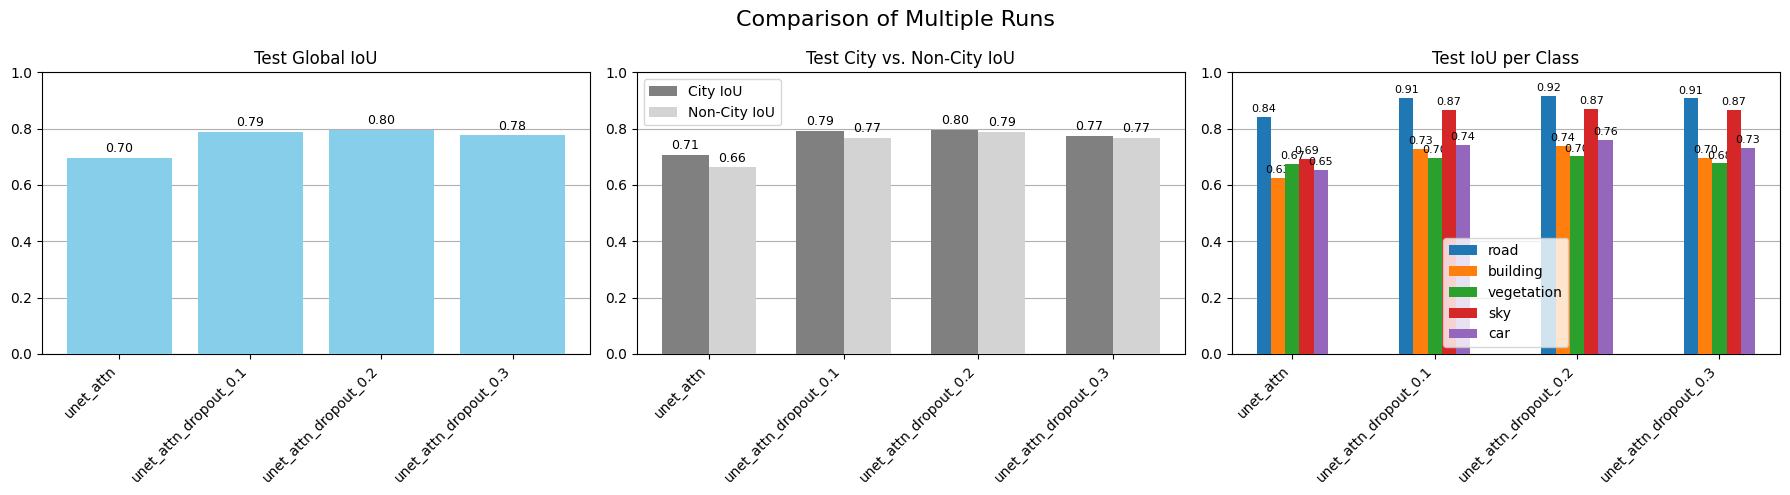
\includegraphics[width=0.8\textwidth]{figures/attention_comparison.png} 
    \caption{Comparison of the Attention U-Net Models.} 
    \label{fig:attention_comparison} 
\end{figure}

At last I also wanted to look at what impact implementing the Attention mechanism could have. There have been some publications like "Crack Semantic Segmentation using the U-Net with
Full Attention Strategy" by Lin et al. \cite{linCrackSemanticSegmentation2021} showing that the attention mechanism can have meaningful impact on the performance of semantic segmentation models. My results did reach a similar IoU ceiling for all recorded scores but upon further visual inspection showed the real strenghts of attention.
\chapter{Reflection}

Reflecting on the work, I found that the dataset presented significant challenges, making the modeling process particularly demanding. Reducing the number of classes provided a meaningful performance boost, yet the presence of numerous "falsely" labeled objects remained a major hurdle, especially for simpler models trying to capture the finer nuances. Despite these challenges, the Attention U-Net exceeded my expectations. Considering the limited data available, I was impressed by how well it performed—especially since attention mechanisms are typically data-hungry. The addition of dropout regularization played a crucial role in further enhancing the Attention U-Net's ability to generalize.

Although the bare metrics suggested that the Attention models performed slightly worse, a closer examination of selected samples convinced me otherwise. The Attention mechanism truly helped the model focus on critical parts of the image, excelling in complex scenes where clarity and confidence in object labeling were vital.

Looking ahead, I see room for further improvements:

\begin{itemize}
    \item Augmenting the dataset to increase the number of training samples
    \item Refining the dataset's ground truths by addressing falsely labeled objects, perhaps by leveraging third-party annotations
\end{itemize}

These steps could help overcome some of the key challenges encountered and further enhance the performance and reliability of the models.

\printbibliography

\end{document}